

Taking the Fourier transform of the field \ref{eq:flux_field}, expanded in terms of the bloch waves
\begin{equation}\label{eq:field_FT}
    \hat{\phi}_n(x, \mu) = \int_{-\infty}^\infty \hat{\phi}_n(x,t) e^{i\mu t} dt
\end{equation}
%
We obtain the following forms for the field at the $n$th CPW segment:
\begin{subequations} \label{eq:phi_FT}
\begin{eqnarray}
    \hat{\phi}_n(x, \mu) =  \left|\left.\frac{d\omega}{dk}\right|_{\omega=\mu}\right|^{-1}\frac{1}{\sqrt{\mu}}\biggl\lbrace \hat{a}_n^R(K) \psi^R_K(x) + \hat{a}_n^L(K)\psi_K^L(x)\biggr\rbrace, & \mu > 0, \label{eq:phi_FT_a}\\
    \hat{\phi}_n(x, \mu) = \left|\left.\frac{d\omega}{dk}\right|_{\omega=\mu}\right|^{-1}\frac{1}{\sqrt{|\mu|}}\biggl\lbrace [\hat{a}^R_n(K)]^\dagger \left[\psi^R_K(x)\right]^* + [\hat{a}_n^L(K)]^\dagger\left[\psi_K^L(x)\right]^*\biggr\rbrace, & \mu < 0. \label{eq:phi_FT_b}
\end{eqnarray}
\end{subequations}
%
Where we use $k_{\mu} = k_{-\mu} = k_{|\mu|}$, $K = |k|$, and the forms of the Bloch functions (see Appendix \ref{ch:Mathematica_KP})

\color{black}

\begin{equation}\label{eq:bloch_waves}
    \psi_{K}^R (x) =e^{iKx} u_{K}^{(1)}(x), \hspace{12pt}  \psi_{K}^L(x) =e^{-iKx} u_{K}^{(2)}(x),
\end{equation}
%
as well as identify operators corresponding to right and left traveling modes
\begin{equation}
    \hat{a}_n(K) = 
    \begin{cases}
    \hat{a}_n^R(K), &\text{if k > 0,}\\
    \hat{a}_n^L(K), &\text{if k < 0.}
    \end{cases}
\end{equation}
%
Taking the Fourier transformed $n$th site boundary condition (\ref{eq:BC_freq_static_unitless_2}) and using our expansion of the field for positive frequencies (\ref{eq:phi_FT}), we arrive at a relation,
%
\begin{equation}\label{eq:BC_static_1}
\begin{split}
    \epsilon \left\lbrace\hat{a}^R(K) \psi^R_K(n) + \hat{a}^L(K) \psi^L_K(n) \right\rbrace =
    \\[2mm]
    \left(\frac{\hbar}{L_0}\right) 
    \left\lbrace\hat{b}^R(K) \left.\frac{\partial \psi^R_K(x)}{\partial x}\right|_{n^-} +\hat{b}^L(K) \left.\frac{\partial \psi^L_K(x)}{\partial x}\right|_{n^-}\right\rbrace
    \\[2mm]
    -
    \left(\frac{\hbar}{L_0}\right) 
    \left\lbrace\hat{a}^R(K) \left.\frac{\partial \psi^R_K(x)}{\partial x}\right|_{n^+} +\hat{a}^L(K) \left.\frac{\partial \psi^L_K(x)}{\partial x}\right|_{n^+} \right\rbrace
\end{split}
\end{equation}
%
Where we have omitted the $n$ subscript in our annihilation/creation operators and defined $\hat{b} = \hat{a}_{n+1}$ (see Fig. \ref{fig:boundary_diagram}).
%
\begin{figure}[h]\label{fig:boundary_diagram}
    \centering
    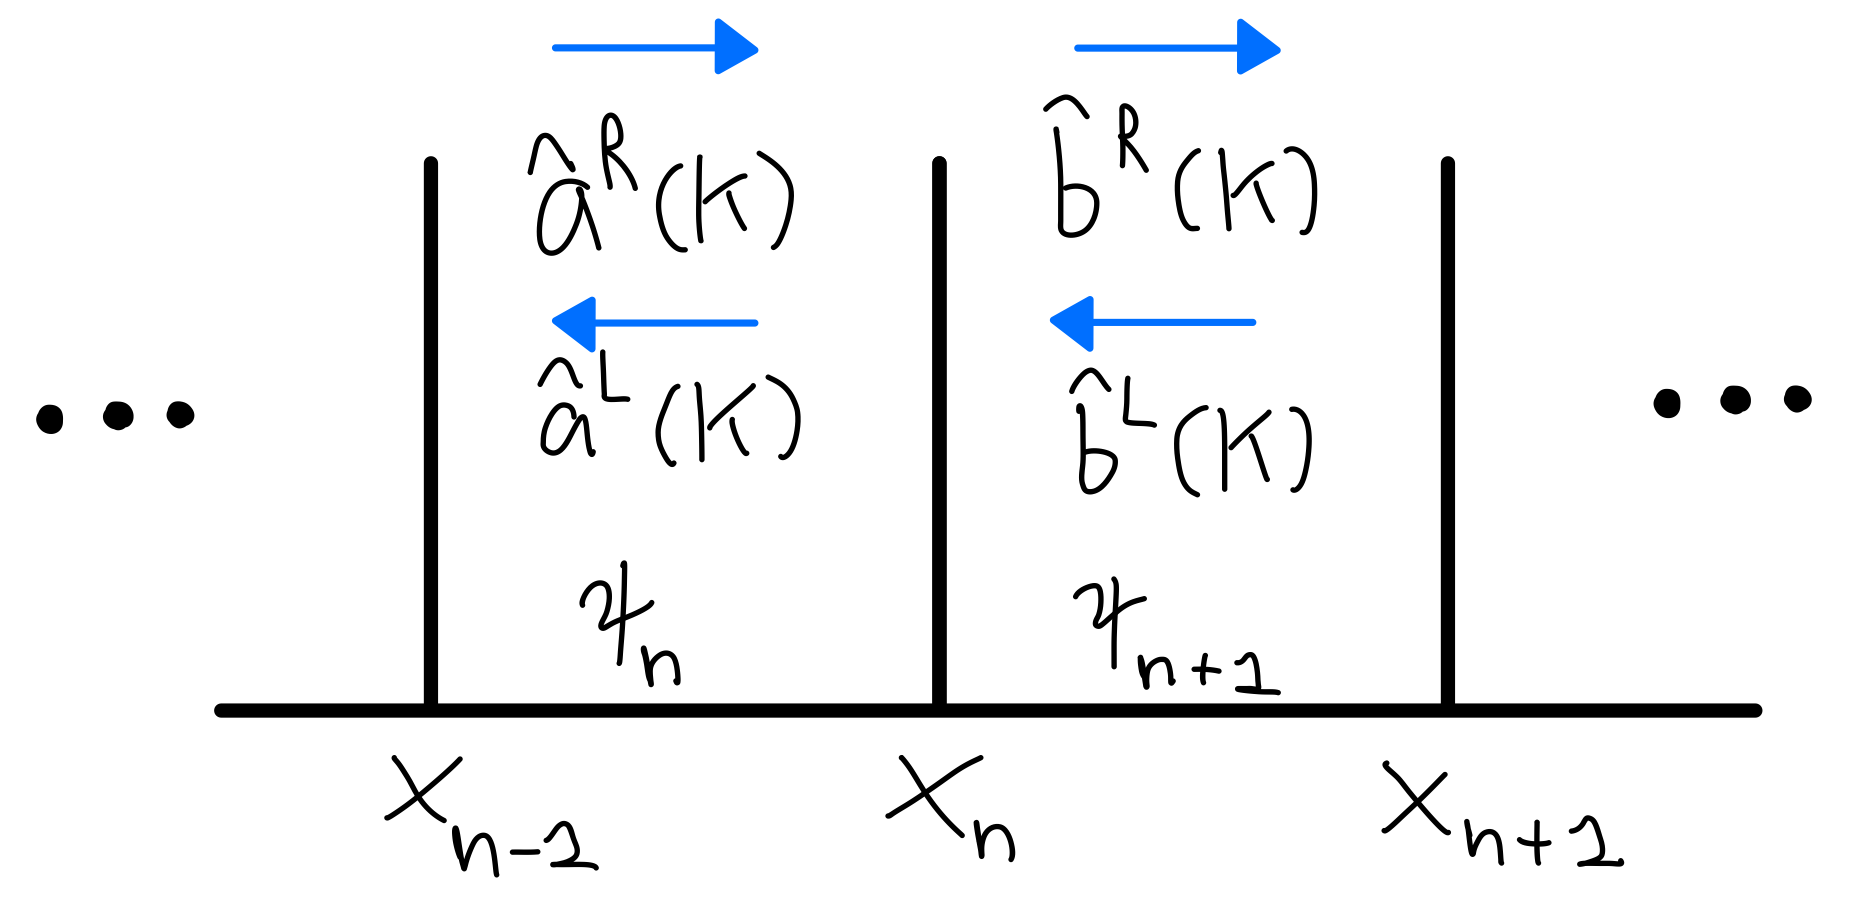
\includegraphics[width=4.5in, keepaspectratio]{figures/boundary_diagram.png}
    \caption{Diagram showing Bloch functions and creation/annihilation operators in the CPWs to the left, and right of SQUID site $n$.}
\end{figure}
%
We use the fact that the Bloch functions $\psi_K(x)$ are, by construction, eigenfunctions of the same boundary condition (\ref{eq:BC_freq_static_unitless_2}) as our field. We can now write our boundary condition in the form
%
\begin{equation}
    \left[\hat{a}^R(K) - \hat{b}^R(K)\right]\left.\frac{\partial \psi^R_K(x)}{\partial x}\right|_{x=n^+}
    +
    \left[\hat{a}^L(K) - \hat{b}^L(K)\right]\left.\frac{\partial \psi^L_K(x)}{\partial x}\right|_{x=n^+} = 0 
\end{equation}
%
Using (eq. \ref{eq:bloch_waves}) and the relation $u_K(x) = u^*_K(x)$ (see Appendix \ref{ch:Mathematica_KP}),
%
\begin{equation}\label{eq:BC_static_2}
\begin{split}
    \left[\hat{a}^R(K) - \hat{b}^R(K)\right]
    \left.
    \left\lbrace
    i K \, u_K(x) + \frac{\partial u_K(x)}{\partial x}
    \right\rbrace
    \,e^{i K x}
    \right|_{x=n}
    \\[2mm]
    +
    \left[\hat{a}^L(K) - \hat{b}^L(K)\right]
    \left.
    \left\lbrace
    -i K\, u_K(x) + \frac{\partial u_K(x)}{\partial x}
    \right\rbrace
    \,e^{-i K x} 
    \right|_{x=n}
    = 0 
\end{split}
\end{equation}
%




For computational convenience, we define notations for the Bloch functions evaluated at the boundary sites $n$
%
\begin{gather}
    \mathcal{C}_K = \left.u_K(x)\right|_{n}
    \label{eq:cal_C}\\
    %
    \mathcal{D}_K = \left.\frac{\partial u_K(x)}{\partial x}\right|_{n}
    \label{eq:cal_D}\\
    %
    \mathcal{A}_K = iK\mathcal{C}_K + \mathcal{D}_K.
    \label{eq:cal_A}
\end{gather}
%
As well as, 
\begin{subequations}\label{eq:cr_an_position_dept}
\begin{eqnarray}
    \hat{a}^R_K(x) = \hat{a}^R(K)\,e^{i K x},
    \\
    \hat{a}^L_K(x) = \hat{a}^L(K)\,e^{-i K x}. 
\end{eqnarray}
\end{subequations}
%
Similarly for $\hat{b}(K)$. We can now write a clean form for our boundary condition using (Eq. \ref{eq:cal_C} - \ref{eq:cr_an_position_dept}),
%
\begin{equation}\label{eq:BC_static_3}
    \left.\left[\hat{a}^R_K(x) - \hat{b}_K^R(x)\right]\right|_{x=n} \mathcal{A}_K
    +
    \left.\left[\hat{a}^L_K(x) - \hat{b}^L_K(x)\right]\right|_{x=n}\mathcal{A}^*_K = 0 
\end{equation}
%
We also impose the requirement that $\hat{\phi}_n(x,\mu)$ is continuous at the boundary $x=n$. Which, using (Eq. \ref{eq:bloch_waves}, we can express as,
%
\begin{equation}\label{eq:continuity_static}
    \left.\left[\hat{a}^R_K(x) + \hat{a}^L_K(x)\right]\right|_{x=n}
    =
    \left.\left[\hat{b}^R_K(x) + \hat{b}^L_K(x)\right]\right|_{x=n}
\end{equation}
%
Using (Eq. \ref{eq:BC_static_3}, \ref{eq:continuity_static}), we arrive at the relations between annihilation coefficients for static applied magnetic flux in our SQUIDs ($E_J(t)= E^0_J$),
%
\begin{subequations}\label{eq:static_solutions}
\begin{eqnarray}
    \hat{b}^R(K) = \hat{a}^R(K),
    \\
    \hat{b}^L(K) = \hat{a}^L(K).
\end{eqnarray}
\end{subequations}
%

Similar equations can be obtained for creation operators by using (Eq. \ref{eq:phi_FT_b}), for $\mu<0$. Note that these solutions imply that photons with allowed frequencies $\mu$, given by the band structure of the lattice (Eq. \ref{eq:bands_condition}), will pass through the whole lattice experiencing only a change in their phase. Meanwhile, photons with frequencies within the band gaps will not pass through the lattice. In this particular sense, behavior of our photons is identical to that of electrons in a solid. Similar treatments with Bloch mode expansions in second-quantization are used in the study of quantum electrodynamics in photonic crystals (see \cite{Gainutdinov2018},\cite{Gainutdinov2021}). The exciting consequences of such treatment in our system come when we consider the dynamic case in the regime where DCE radiation is generated.


%%%%%%%%%%%%%%%%%%%%%%%%%%%%%%%%%%%%%%%%%%%%%%%%%%%%%%%%%%%%%%%%%%%%%%%%%%%%%%%%%%%%%%%%%%%%%%%%%%%%%%%%%%%%%%

% \section{Dynamical Casimir radiation in the periodic SQUID array}\label{sec:dcr}


We now wish to analyze the dynamic version of our system, where the potential now exhibits a time dependent modulation. We use the results obtained for the static case (Eq. \ref{eq:cal_C} - \ref{eq:BC_static_3}) to write the Fourier-transformed boundary condition (Eq. \ref{eq:BC_field}) for a time-dependent Josephson energy $E_J(t)$,
%
\begin{equation}\label{eq:BC_time_dependent}
\begin{split}
    \left(\frac{\hbar}{L_0}\right)
    \frac{d\omega(K)}{\sqrt{\mu}}
    \left\lbrace
    \left.
    \left[\hat{a}^R_K(x) - \hat{b}_K^R(x)\right]
    \right|_{x=n}
    \mathcal{A}_K +
    \left.
    \left[\hat{a}^L_K(x) - \hat{b}^L_K(x)\right]
    \right|_{x=n}
    \mathcal{A}^*_K
    \right\rbrace
    \\[4mm]
    +\hspace{2mm}
    \hbar \, \left(\frac{2\pi}{\Phi_0}\right)^2
    %
    \left[
    \int_{0}^{\infty} dK'\,
    \delta g(K, K')
    \left.
    \left\lbrace \hat{a}^R_K(x) + \hat{a}_K^L(x) \right\rbrace
    \right|_{x=n}
    \mathcal{C}_K\right.
    \\[4mm]
    +
    \left.
    \int_{-\infty}^{0} dK'\,
    \delta g(K, K')
    \left.
    \left\lbrace [\hat{a}^R_K(x)]^\dagger + [\hat{a}_K^L(x)]^\dagger \right\rbrace
    \right|_{x=n}
    \mathcal{C}_K
    \right]
    = 0
    %
\end{split}
\end{equation}
%
Where we have made a change of variables to so that integration runs over $K'=K(\mu')$, separated the integral into two sections, (for positive and negative $\mu$), and defined the following
%
\begin{gather}
    d\omega (K) = 
    \left|\left.\frac{d\omega}{dK}\right|_{\omega=\mu}\right|^{-1}
    \label{eq:shorthand_dw}
    \\
    \delta g(\mu, \mu') = \frac{1}{2 \pi} \sqrt{\frac{|\mu|}{|\mu'|}}
    \int_{-\infty}^{\infty} dt \, \epsilon(t) \, e^{i(\mu - \mu')t}
    \label{eq:energy_FT}
    \\
    g(\mu, \mu') =  \frac{1}{2 \pi} \sqrt{\frac{|\mu|}{|\mu'|}}
    \int_{-\infty}^{\infty} dt \, E_J(t) \, e^{i(\mu - \mu')t}
    = E_J^0 + \delta g(\mu, \mu').
\end{gather}
%
We proceed to drive our system by applying an external flux equally to all of the SQUID sites, such that the form of the time-dependent Josephson energy (Eq. \ref{eq:energyexp1}), where the drive is in phase $\varphi_n=0$ is:
%
\begin{equation}\label{eq:time_dependent_energy}
\begin{split}
    E_J(t) = E^0_J + \epsilon(t),
    \\
    \text{where,} \hspace{2mm}
    \epsilon(t) = \delta E^0_J \cos(\Omega t). 
\end{split}
\end{equation}
%
We consider a weak harmonic drive, such that $\frac{\delta E^0_J}{E^0_j} \ll 1$. Then, the
%
\begin{equation}
    \delta g(\mu, \mu') =
    \frac{\delta E_J^0}{2}
    \sqrt{\frac{|\mu|}{|\mu'|}}
    \left[
    \delta (\mu' - \mu - \Omega) +
    \delta(\mu' - \mu + \Omega)
    \right]
\end{equation}
%
or, in terms of $K$,
\begin{equation} \label{eq:dw_K_continuous}
    \delta g(K,K')= 
    \frac{\delta E_J^0}{2}
    \sqrt{\frac{|\mu|}{|\mu'|}}
    d\omega (K')
    \left[
    \delta (K' - K_+) + \delta(K' - K_-)
    \right]
\end{equation}
% 
where we have used the shorthand notations,
%
\begin{gather}
    K_+ = K(\mu + \Omega),\\
    %
    K_- = K(\mu - \Omega).
\end{gather}
%

\subsection{Numerical Calculation: Band Structure, and Reduced Domains}

In order to obtain a transfer matrix for our system, we need a relation between operators right and left of our boundary. To do this we use our boundary condition (Eq. \ref{eq:BC_time_dependent}), truncate the frequency range to $[-\Omega, \Omega]$ and discretizing it in $(2 N_{\Omega} + 1)$ steps $[-\omega_N, ..., \omega = 0, ..., \omega_N]$ where $\omega_N = \Omega$. 

We parametrize as $\omega_n = \omega + (N_{\Omega} + 1 - n)$, where $n = 1, ..., 2N_{\Omega}+1$, and define $K_n = K(|\omega_n|)$, $d \omega (n) = d \omega(K_n)$, similarly for $\mathcal{A}_n = \mathcal{A}_{K_n}, \mathcal{C}_n = \mathcal{C}_{K_n}$. We can now write, 
%
\begin{equation}\label{eq:BC_discrete_1}
\begin{split}
    \left(\frac{1}{L_0}\right)
    d\omega(n)
    \left\lbrace
    \left[\hat{a}_R(n) - \hat{b}_R(n)\right]
    \mathcal{A}_n 
    +
    \left[\hat{a}_L(n) - \hat{b}_L(n)\right]
    \mathcal{A}^*_n
    \right\rbrace
    \\[4mm]
    +\hspace{2mm}
    \left(\frac{2\pi}{\Phi_0}\right)^2
    %
    \left[
    \sum_{m=-N}^{N} \Delta K_m\,
    \delta g_{m, n}
    d \omega(m)
    \left\lbrace \hat{a}_R(m) + \hat{a}_L(m) \right\rbrace
    \mathcal{C}_m\right.
    \\[4mm]
    +
    \left.
    \sum_{m=-N}^{N} \Delta K_m\,
    \delta g_{m, n}
    d \omega(m)
    \left\lbrace [\hat{a}_R(m)]^\dagger + [\hat{a}_L(m)]^\dagger \right\rbrace
    \mathcal{C}_m
    \right]
    = 0
    %
 \end{split}
\end{equation}
%
\begin{equation}
    \delta g(n,m)= 
    \frac{\delta E_J^0}{2}
    \sqrt{\frac{|\omega_n|}{|\omega_m|}}
    \left[ 
    d\omega (n+1) \delta_{m, n+1}
    + d\omega (n-1) \delta_{m, n-1}
    \right]
\end{equation}
%
Multiplying both sides by $\left(\frac{\Phi_0}{2\pi}\right)^2 \frac{1}{E_J^0}$ and using 
\begin{equation}
    L_{\text{eff}} = \left(\frac{\Phi_0}{2\pi}\right)^2 \frac{1}{E_J^0 L_0}
\end{equation}
%

\begin{comment}
\begin{equation}\label{eq:BC_discrete_2}
\begin{split}
    L_{\text{eff}}\, 
    d\omega(n)
    \left\lbrace
    \left[\hat{a}_R(n) - \hat{b}_R(n)\right]
    \mathcal{A}_n 
    +
    \left[\hat{a}_L(n) - \hat{b}_L(n)\right]
    \mathcal{A}^*_n
    \right\rbrace
    \\[4mm]
    +\hspace{2mm}
    \frac{\delta E_J^0}{2 E_J^0}
    %
    \sum_{m=1}^{2N_{\Omega}+1}
    \sqrt{\frac{|\omega_n|}{|\omega_m|}}
    d \omega(m)
    \left[ 
    \delta_{m, n+1}
    + \delta_{m, n-1}
    \right]
    \\[4mm]
    *
    \left[
    \Theta(\omega_n)
    \left\lbrace \hat{a}_R(m) + \hat{a}_L(m) \right\rbrace
    \mathcal{C}_m
    +
    \Theta(-\omega_n)
    \left\lbrace [\hat{a}_R(m)]^\dagger + [\hat{a}_L(m)]^\dagger \right\rbrace
    \mathcal{C}_m
    \right]
    = 0
    %
 \end{split}
\end{equation}
\end{comment}


